% chktex-file 3 chktex-file 9 chktex-file 10 chktex-file 17 chktex-file 18 chktex-file 36 chktex-file 40
\section*{Exercise 1.3.}

Suppose that $m_t = c_0 + c_1 t + c_2 t^2,\; t = 0,\pm 1,\ldots$
\begin{enumerate}[label=(\alph*)]
    \item Show that
    \[ m_t = \sum_{i = -2}^{2}a_i m_{t+i} = \sum_{i = -3}^{3}b_i m_{t+i},\hspace{2em} t = 0,\pm1,\ldots, \]
    where $a_2 = a_{-2}=-\frac{3}{35}$, $a_1 = a_{-1}=\frac{12}{35}$, $a_0 = \frac{17}{35}$, and $b_3 = b_{-3} = -\frac{2}{21}$, $b_2 = b_{-2} = \frac{3}{21}$, $b_1 = b_{-1} = \frac{6}{21}$, $b_0 = \frac{7}{21}$.
    \item Suppose that $X_t = m_t + Z_t$ where $\{Z_t, t = 0,\pm 1,\ldots\}$ is an independent set of normal random variables, each with mean 0 and variance $\sigma^2$. Let $U_t = \sum_{i = -2}^2 a_i X_{t+i}$ and $V_t = \sum_{i = -3}^3 b_i X_{t+i}$.
    \begin{enumerate}[label=(\roman*)]
        \item Find the means and variances of $U_t$ and $V_t$.
        \item Find the correlations between $U_t$ and $V_t$.
        \item Which of the two filtered series $\{U_t\}$ and $\{V_t\}$ would you expect to be smoother in appearance?
    \end{enumerate}
\end{enumerate}

\subsection*{Solution Part (a)}

In the first place, note that since $a_i = a_{-i}$ and $b_i = b_{-j}$, it follows that

\[ \sum_j a_j m_{t+j} =  \sum_j a_j m_{t-j}, \]
\[ \sum_j b_j m_{t+j} =  \sum_j b_j m_{t-j}. \]
The same goes for $U_t$ and $V_t$.

We use the lemma from the previous exercise to prove that the filters $\{a_j\}$ and $\{b_j\}$ don't distort quadratic polynomials.

\begin{figure}[H]
    \centering
    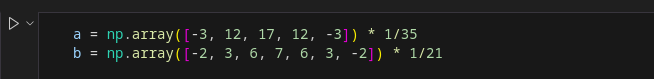
\includegraphics[width=0.85\textwidth]{../pictures/hw1ex1.3.0.png}
\end{figure}

\[ \sum_{j = -2}^2 a_j j^r = \begin{cases}
    1, & r = 0\\
    0, & r = 1,2
\end{cases} \]

\begin{figure}[H]
    \centering
    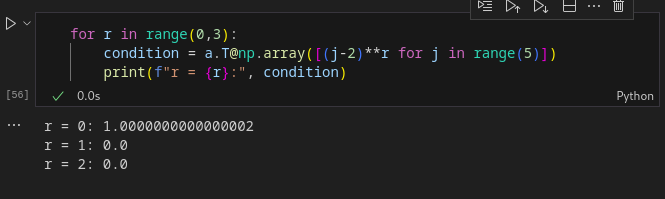
\includegraphics[width=0.85\textwidth]{../pictures/hw1ex1.3.1.png}
\end{figure}

\[ \sum_{j = -3}^3 b_j j^r = \begin{cases}
    1, & r = 0\\
    0, & r = 1,2
\end{cases} \]

\begin{figure}[H]
    \centering
    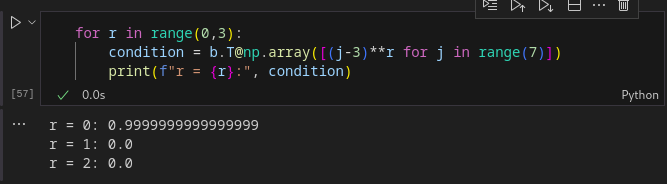
\includegraphics[width=0.85\textwidth]{../pictures/hw1ex1.3.2.png}
\end{figure}

Therefore, 
\[ m_t = \sum_{j = -2}^2 a_j j^r = \sum_{j = -3}^3 b_j j^r. \]

\subsection*{Solution Part (b)}

\textbf{Item (i):} By linearity,
\[ \everymath{\displaystyle}
\arraycolsep=1.8pt\def\arraystretch{2.5}
\begin{array}{rcl}
    U_t = \sum_{i = -2}^2 a_i X_{t-i} & = & \sum_{i = -2}^2 a_i m_{t-i} + \sum_{i = -2}^2 a_i Z_{t-i}\\
    & = & m_t + \sum_{i = -2}^2 a_i Z_{t-i}
\end{array} \]
\[ \implies \E U_t = \E m_t + \sum_{i = -2}^2 a_i \E Z_{t-i} = m_t + 0. \] 
\[ \implies \Var U_t = \Var m_t + \sum_{i = -2}^2 a_i \Var Z_{t-i} = 0 + \sigma^2 \sum_{i = -2}^2 a_i = \sigma^2 . \] 
If we do the same with $V_t$, then we obtain $\E V_t = m_t$ and $\Var V_t = \sigma^2$

\textbf{Item (ii):}
\[ \everymath{\displaystyle}
\arraycolsep=1.8pt\def\arraystretch{2.5}
\begin{array}{rcl}
    \sigma^2 \corr(U_t,V_t) & = & \E[(U_t-m_t)(V_t - m_t)]\\
    & = & \E(U_t V_t) - m_t\E U_t - m_t\E V_t + \E m_t^2\\
    & = & \E \left[ \left( m_t + \sum_{i = -2}^2 a_i Z_{t-i} \right) \left( m_t + \sum_{i = -3}^3 b_i Z_{t-i} \right) \right] - m_t^2\\
    & = & \E\left( m_t^2 + m_t \sum_{i = -2}^2 a_i Z_{t-i} + m_t \sum_{i = -3}^3 b_i Z_{t-i} + \sum_{i = -2}^2 a_i Z_{t-i} \sum_{i = -3}^3 b_i Z_{t-i} \right) - m_t^2\\
    & = & m_t + 0 + 0 + \E\left( \sum_{i = 0}^4 a_{i-2} Z_{t-i+2} \sum_{i = 0}^6 b_{j-3} Z_{t-j+3} \right) - m_t^2\\
    & = &  \sum_{k = 0}^{\infty} \sum_{j = 0}^k a_{j-2} b_{k-j-3} \E Z_{t-j+2} Z_{t-k+j+3}
\end{array}\]
Then, $\E Z_{t-j+2} Z_{t-j+k+3} = \sigma^2$ when $t-j+3 = t-k+j+3$ and 0 otherwise, and that is when $2j = k$. Thus,
\[ \everymath{\displaystyle}
\arraycolsep=1.8pt\def\arraystretch{1.5}
\begin{array}{rcl}
    \corr(U_t,V_t) & = & \frac{\sigma^2}{\sigma^2} \sum_{k/2 \in \N_0} \sum_{j = k/2}^{k/2} a_{k-2} b_{k-j-3} \\
    & = & \sum_{k = 0}^{\infty} a_{k-2} b_{k-3}\\
    & = & a_{-2}b_{-3} + a_{-1}b_{-2} + a_{0}b_{-1} + a_{1}b_{0} + a_{2}b_{1}\\
    & \approx & 0.286
\end{array} \]

\textbf{Item (iii):} $V_t$ should be smoother because $\{b_t\}$ is a weighted average of more elements and $b_0$ weights a 3rd of the total average. On the other hand, $a_0$ weights almost half of this sum, so $Z_t$ has more influence in $U_t$ than in $V_t$.